%
\section{Semantic and Visual Clustering}
\label{sec_inhalt}

The nodes received through the tree-based search are potentially very large (i.e., many pictures were found for the node). We found a rather small semantic and a large visual diversity within these nodes. It is therefore appropriate to refine especially the large nodes into smaller clusters.

\subsection{General Approach}
Since semantics are more meaningful to humans, and thus likely to be more important for the given use case, the refinement is done first on a semantic and then on a visual basis. That is, the results from the groups with semantically similar pictures are clustered again into subclusters with visually similar pictures. The steps are explained in more detail in sections \ref{sec_keywordclustering} and \ref{sec_visualclustering}.
This approach has the additional advantage that outlier images, which have been assigned to a node but do not quite fit with the others because they show something different, can be filtered out in the semantic step. \\
The subclustering explained below and summarized in figure \ref{fig_semanticandvisual} will only take place for nodes/clusters with a certain minimum size and results in the structure of three nested Arrays of the WordnetNode class' attribute \emph{subclusters} shown in figure \ref{fig_nodestructure}.

\begin{figure}[h]
\centering
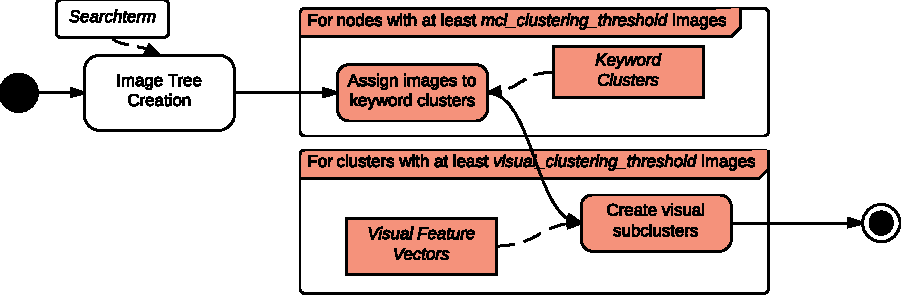
\includegraphics[width=\textwidth]{images/semantic_and_visual_clustering.pdf}
\caption{Process of Semantic and Visual Clustering}
\label{fig_semanticandvisual}
\end{figure}

The data structures used in the process, such as Image Lookup Structures and Visual Feature Vectors, need only be calculated once for each image set. The preparational processes are visualized by figure \ref{fig_precalcprocess}.

\begin{figure}[h]
\centering
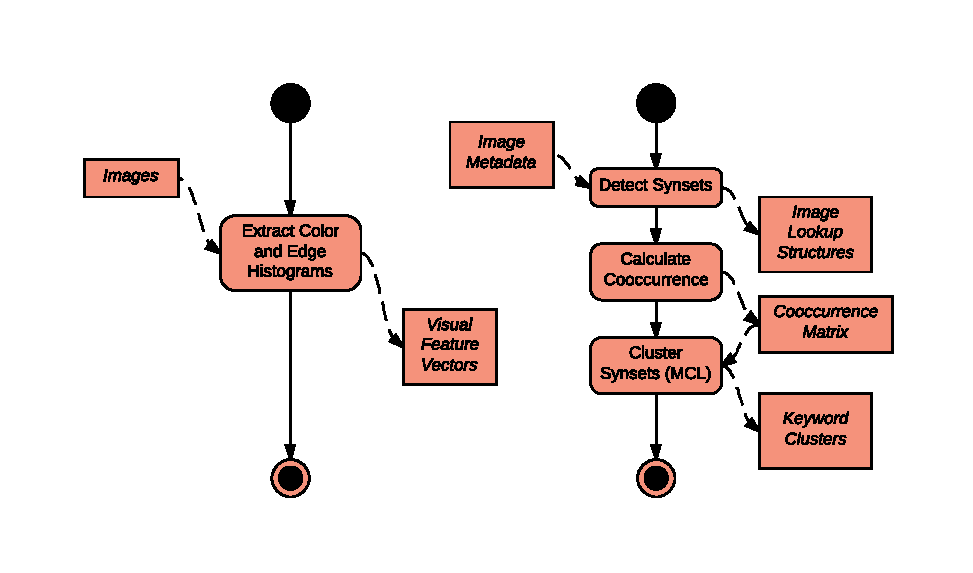
\includegraphics[width=0.8\textwidth]{images/precalcs_activity_diagram.pdf}
\caption{Static structures creation processes}
\label{fig_precalcprocess}
\end{figure}


\subsection{Keyword Clusters}
\label{sec_keywordclustering}
Semantic clustering is accomplished by using the associated Synsets which the Synset detection assigned to each image (see chapter \ref{sec_synsetdetection}). Therefore, Synsets are clustered into groups and images are assigned to these groups.

\bigskip
According to the paper ``Automated Tag Clustering'' by Grigory Begelman \cite{begelman2006automated}, our first approach of clustering Synsets used co-occurrences to span a graph of related Synsets. This graph consists of nodes representing the Synsets and edges representing the number of co-occurrences between Synsets. To include the advantages of Wordnet in the graph, we decided to replace the number of co-occurrences by a combination of co-occurrences and LCH-Similarity\index{LCH-Similarity}. The paper describes a graph clustering algorithm to achieve a grouping of related Synsets. But, the algorithm requires calculation of eigenvalues and eigenvectors for large sparse matrices. Furthermore, it does not take edge weighting into account. Consequently, we replace the graph clustering algorithm by the Markov Cluster Algorithm (MCL)\index{Markov Cluster Algorithm} introduced by Dongen \cite{Dongen1998}. MCL is based on the Random Walk Model \cite{spitzer2001principles}. The basic idea is, if you start to walk from a node, it is more likely to stay inside a cluster than to leave it. Therefore, we calculate the probability to reach a node $B$ from another node $A$ in only one step. Then, we walk steps through the graph until the probabilities converge. The resulting probabilities inside a cluster are higher than outside. So, they can be used to determine groups of related Synsets.\\

\bigskip
To assign images to Synset clusters, we count how many Synsets the image shares with each cluster. It is then assigned to the cluster with the most matching Synsets. If two clusters have the same number of matching Synsets, the image is assigned to both clusters. As a consequence, a semantic cluster consists of images which have many associated Synsets in the same Synset cluster. For example, some pictures with parrots fall into a Synset cluster with persons, others in those with trees.\\

\bigskip
The advantages of an additional semantic clustering in each node of the image tree are obvious when looking at ``Africa'' as search term. The spanned tree consists of part-meronyms which are the countries of Africa. However, the pictures show people, animals, vegetation, cities, or other content not related solely to Africa. Simply with the help of the image tree, it is not possible to separate between those categories. Semantic clustering, allows in this context a more fine grained clustering. Also, in a well separated tree it is possible to achieve a more fine grained clustering. Pictures of the tree node \emph{parrot.n.01} could be separated into pictures showing parrots in nature and pictures showing parrots in a zoo. Furthermore, semantic clustering permits the detection of outliers. If too few images fall into the same semantic cluster, they are considered to be outliers, and they are deleted from the tree node. For instance, a picture showing a cat whose name is ``Alexandria'', which is a city in Africa, can be deleted from the tree for the search term ``Africa''.

\subsection{Visual Clusters}
\label{sec_visualclustering}

One difficulty in the visual part of our work, besides the choice of appropriate features and their implementation, is the question how to use them jointly in a suitable algorithm for clustering.

\subsubsection{Features}
The features we chose for our tool are:
\begin{itemize}
\item{Color histogram} in HSV color space with 20 bins (i.e., 20 ranges) each
\item{Edge histogram} length and angle histograms with 10 bins (i.e., 10 different angles considered) as combined vector 
\end{itemize}
The reasons we chose these are that they are easy to calculate, rather obvious and humanly comprehensible. Since the purpose of this visual clustering is only in refining the semantic clusters, and not in trying to distinguish concepts by visual features, there is no apparent need for the use of more complex features.\\
For feature extraction, we use a pyramidal approach similar to the one proposed in \cite{Lazebnik2006}. Its advantage is that it combines features extracted over the entire image with features extracted on separate regions. The advantage of splitting images into regions for feature extraction is that, for example, two images with the same colors but in different structures will not automatically have the same color feature vectors (as visualized in figure \ref{fig_blackwhite}). At the same time, the images' structure gains an unproportionally high importance, especially when using a large number of regions. When using 5x5 rectangles, for example, it can be observed that images with same-colored borders were considered very similar, independent of their actual content.\\

\begin{figure}[h]
\centering
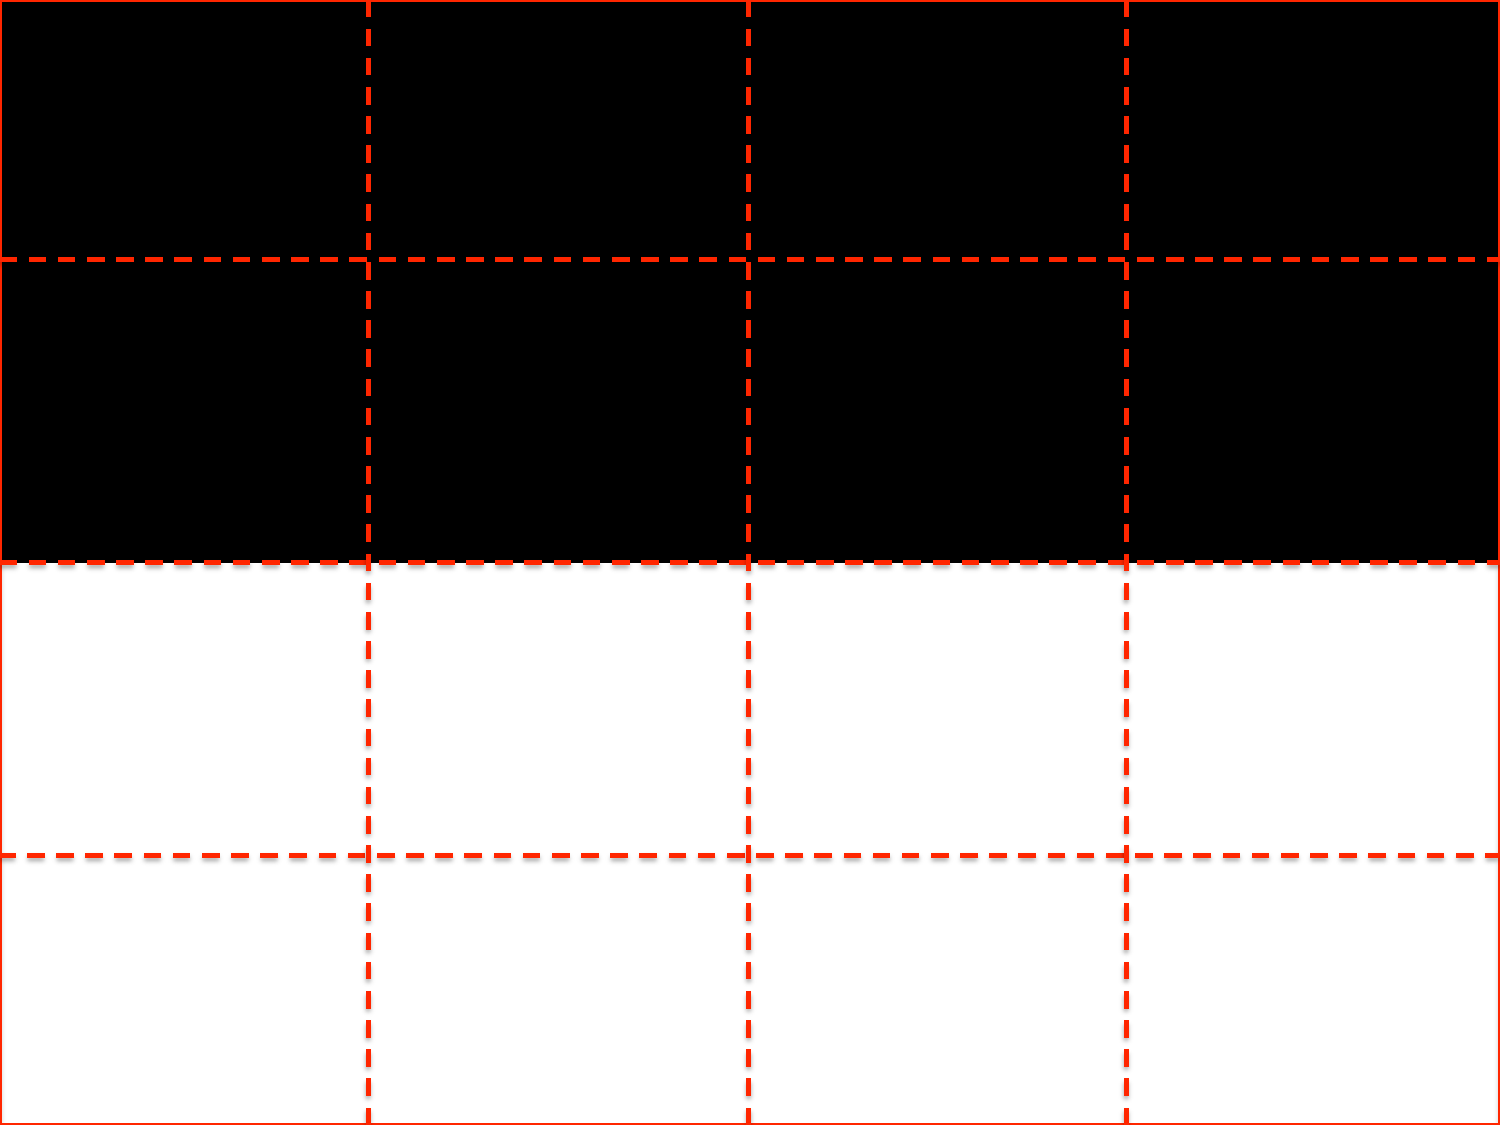
\includegraphics[width=0.35\textwidth]{images/blackwhite1.pdf}
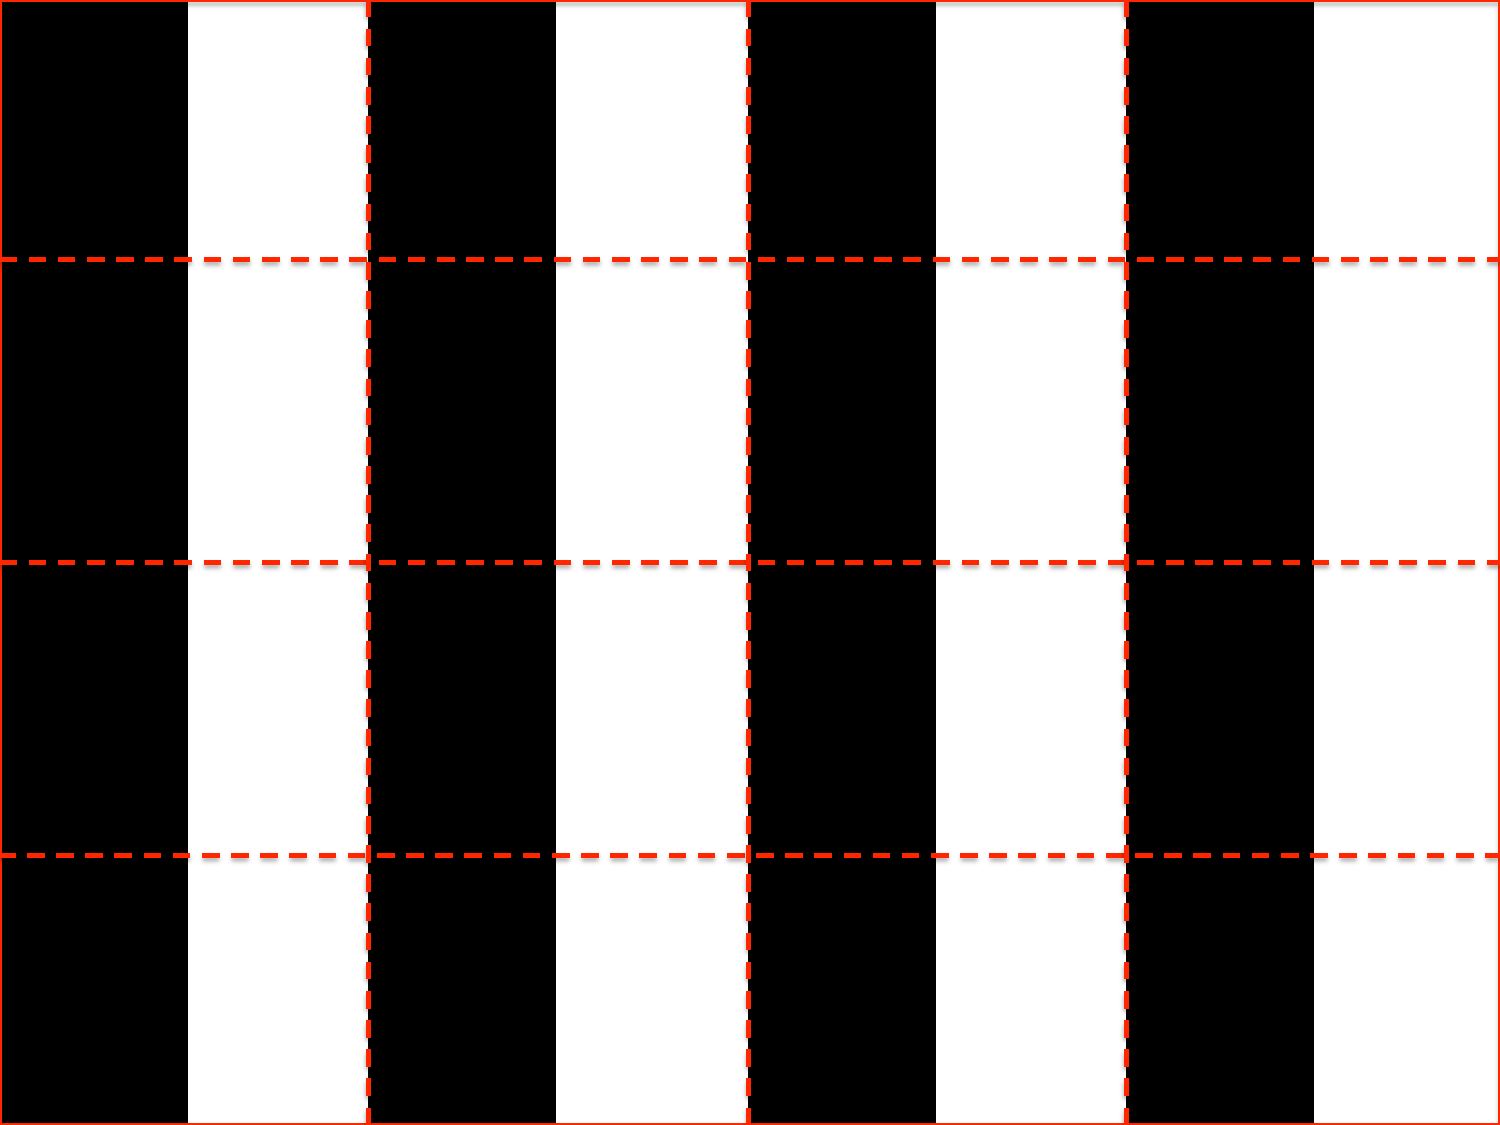
\includegraphics[width=0.35\textwidth]{images/blackwhite2.pdf}
\caption{Two images that have the same color histogram regarding the entire picture but different histograms on the marked regions}
\label{fig_blackwhite}
\end{figure}

With the applied pyramid technique, the final feature vector is concatenated from several partial feature vectors, labeled from 1 to 30 in figure \ref{fig_blackwhite}. The appropriateness of this method especially for refining existing clusters, is also discussed in \cite{Lazebnik2006}. 

\begin{figure}[h]
\centering
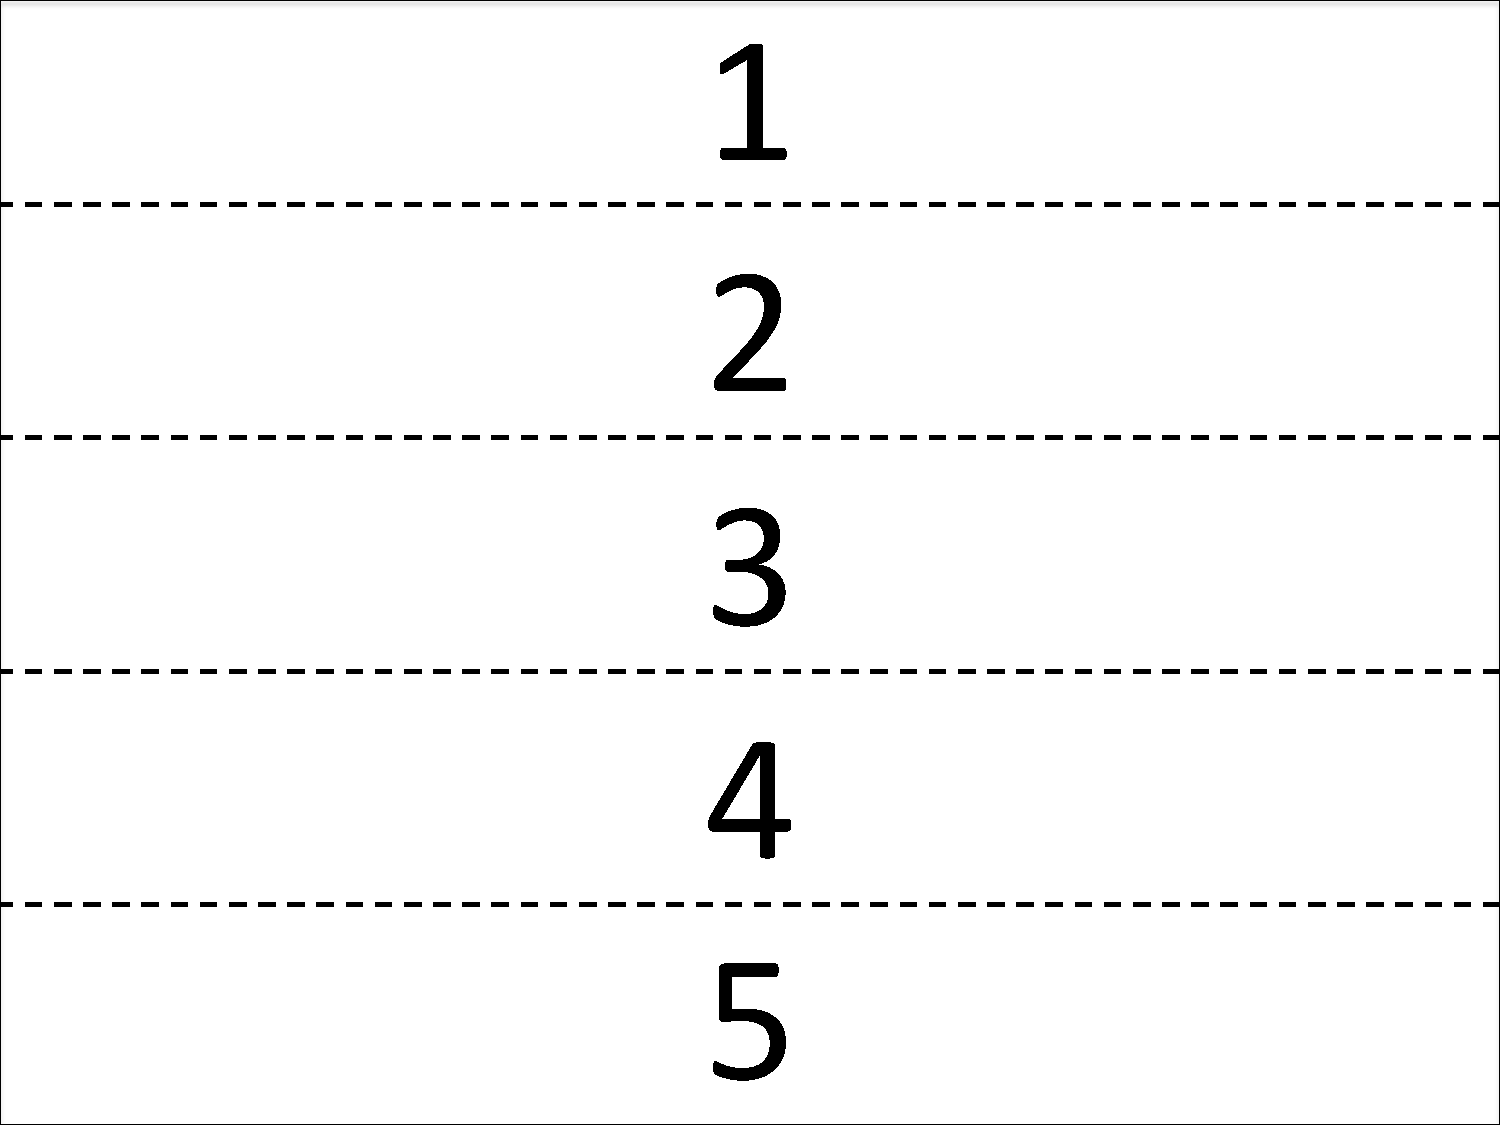
\includegraphics[width=0.19\textwidth]{images/partitioning5h.pdf}
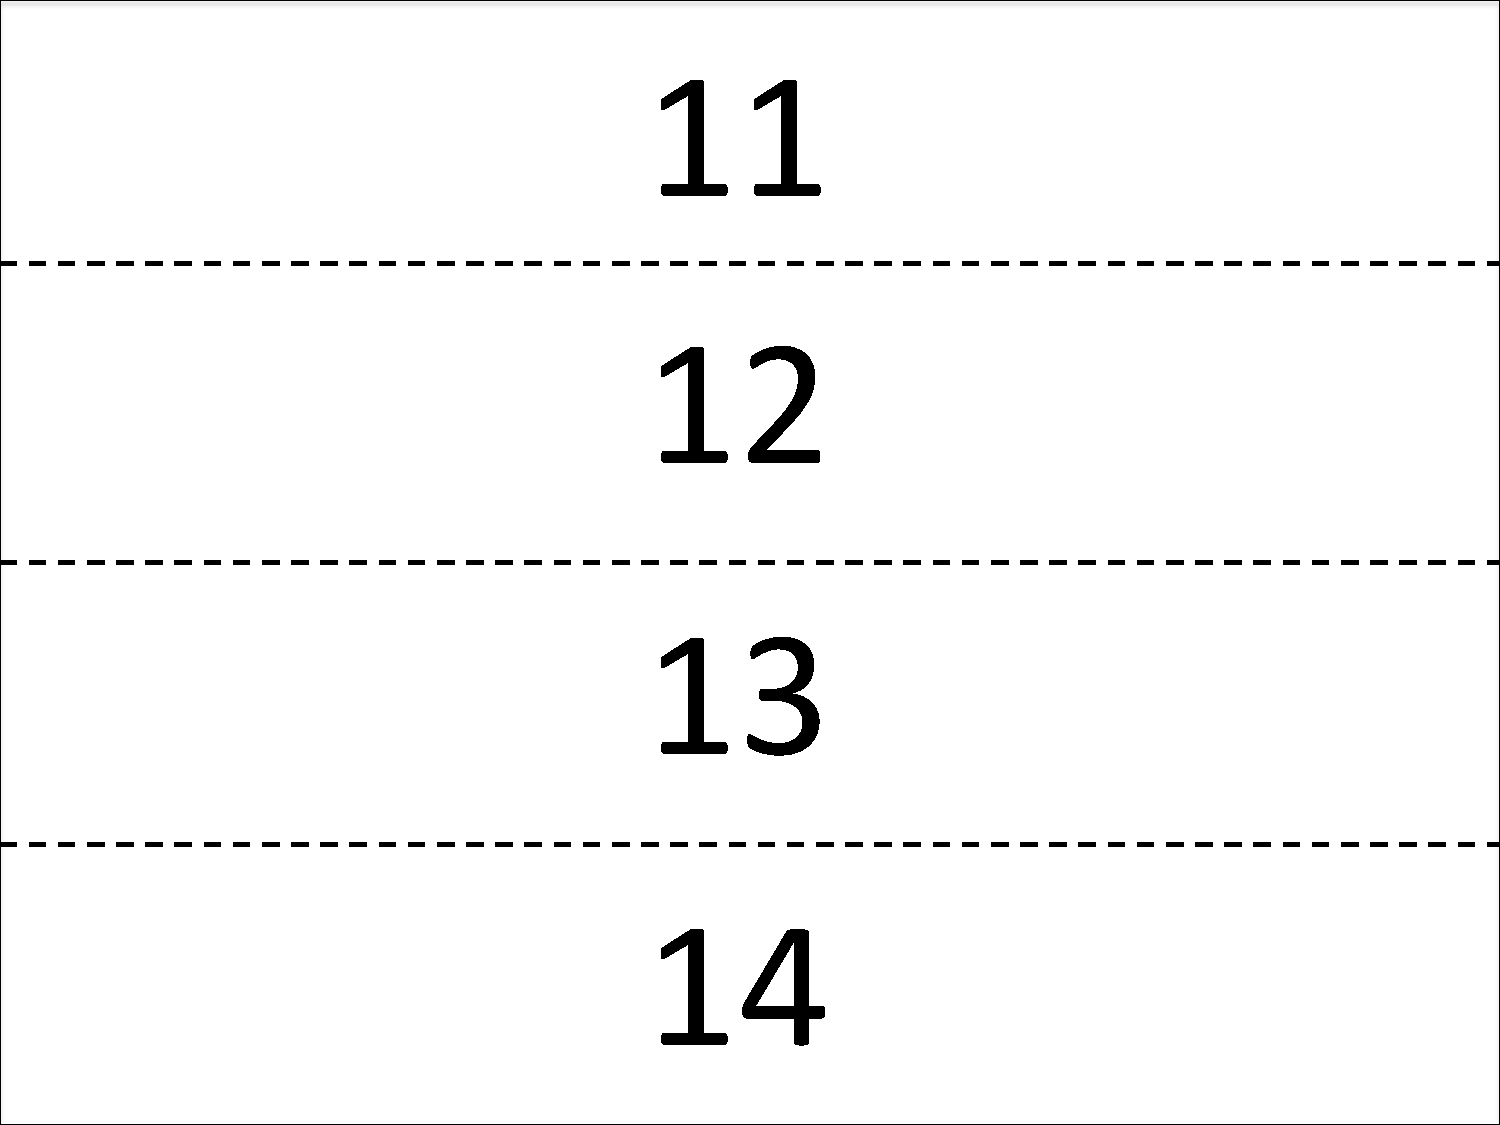
\includegraphics[width=0.19\textwidth]{images/partitioning4h.pdf}
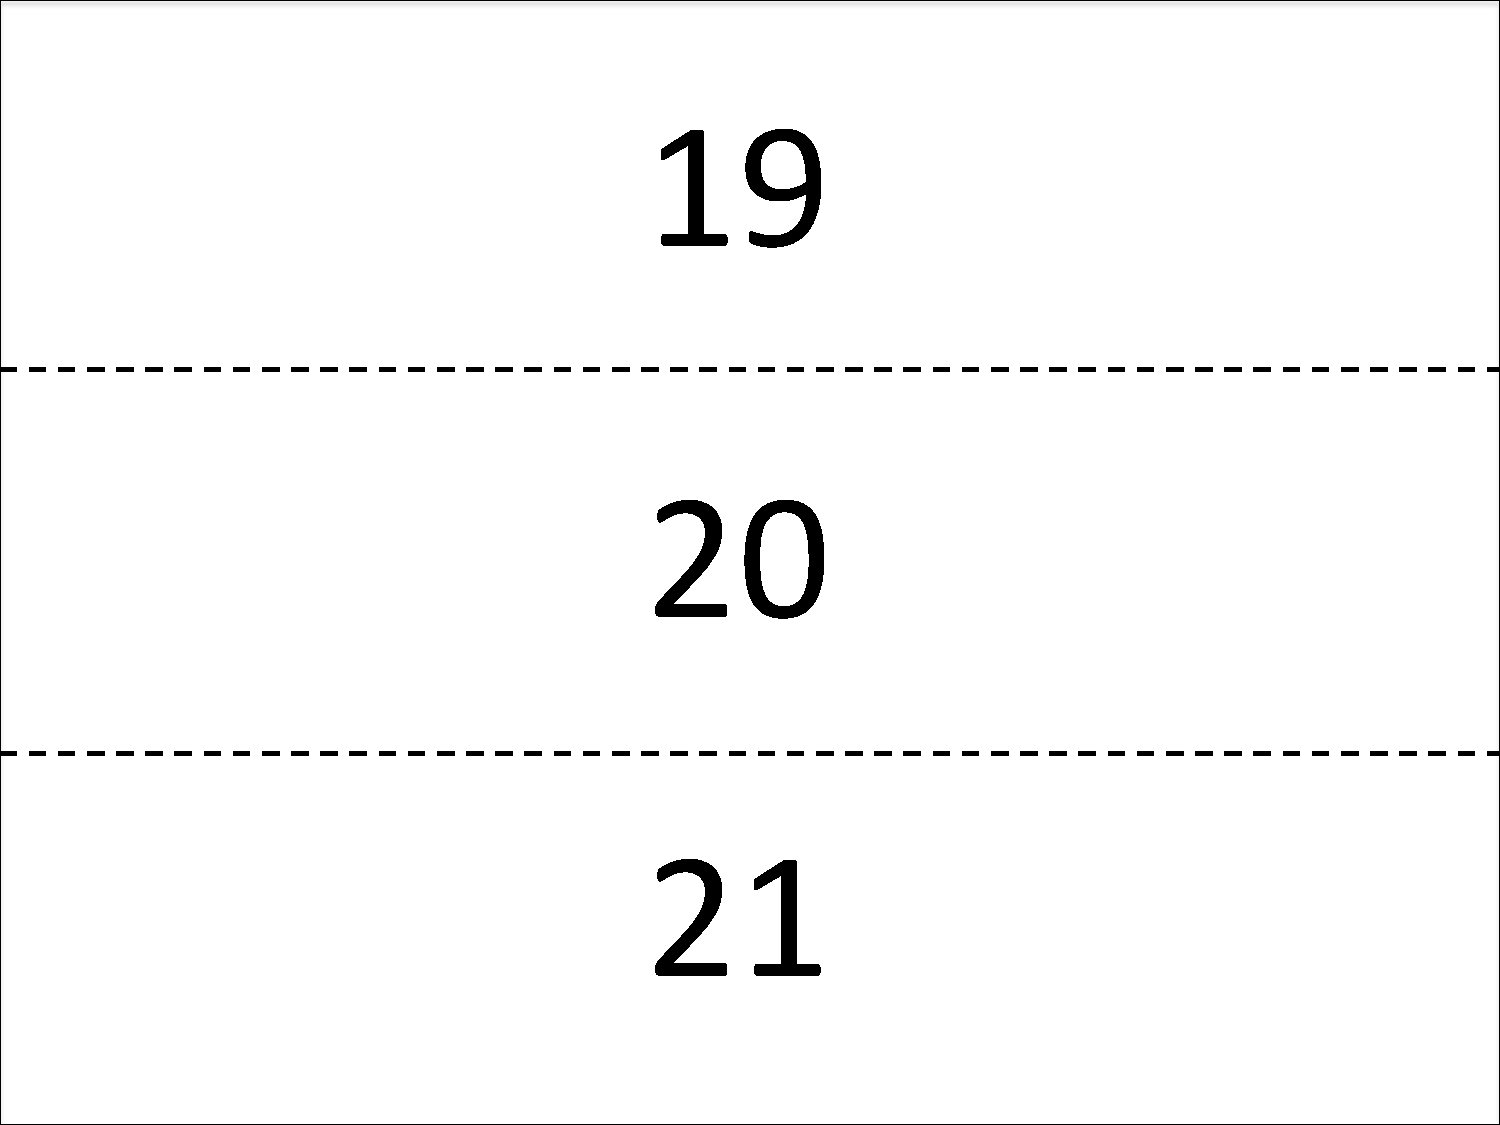
\includegraphics[width=0.19\textwidth]{images/partitioning3h.pdf}
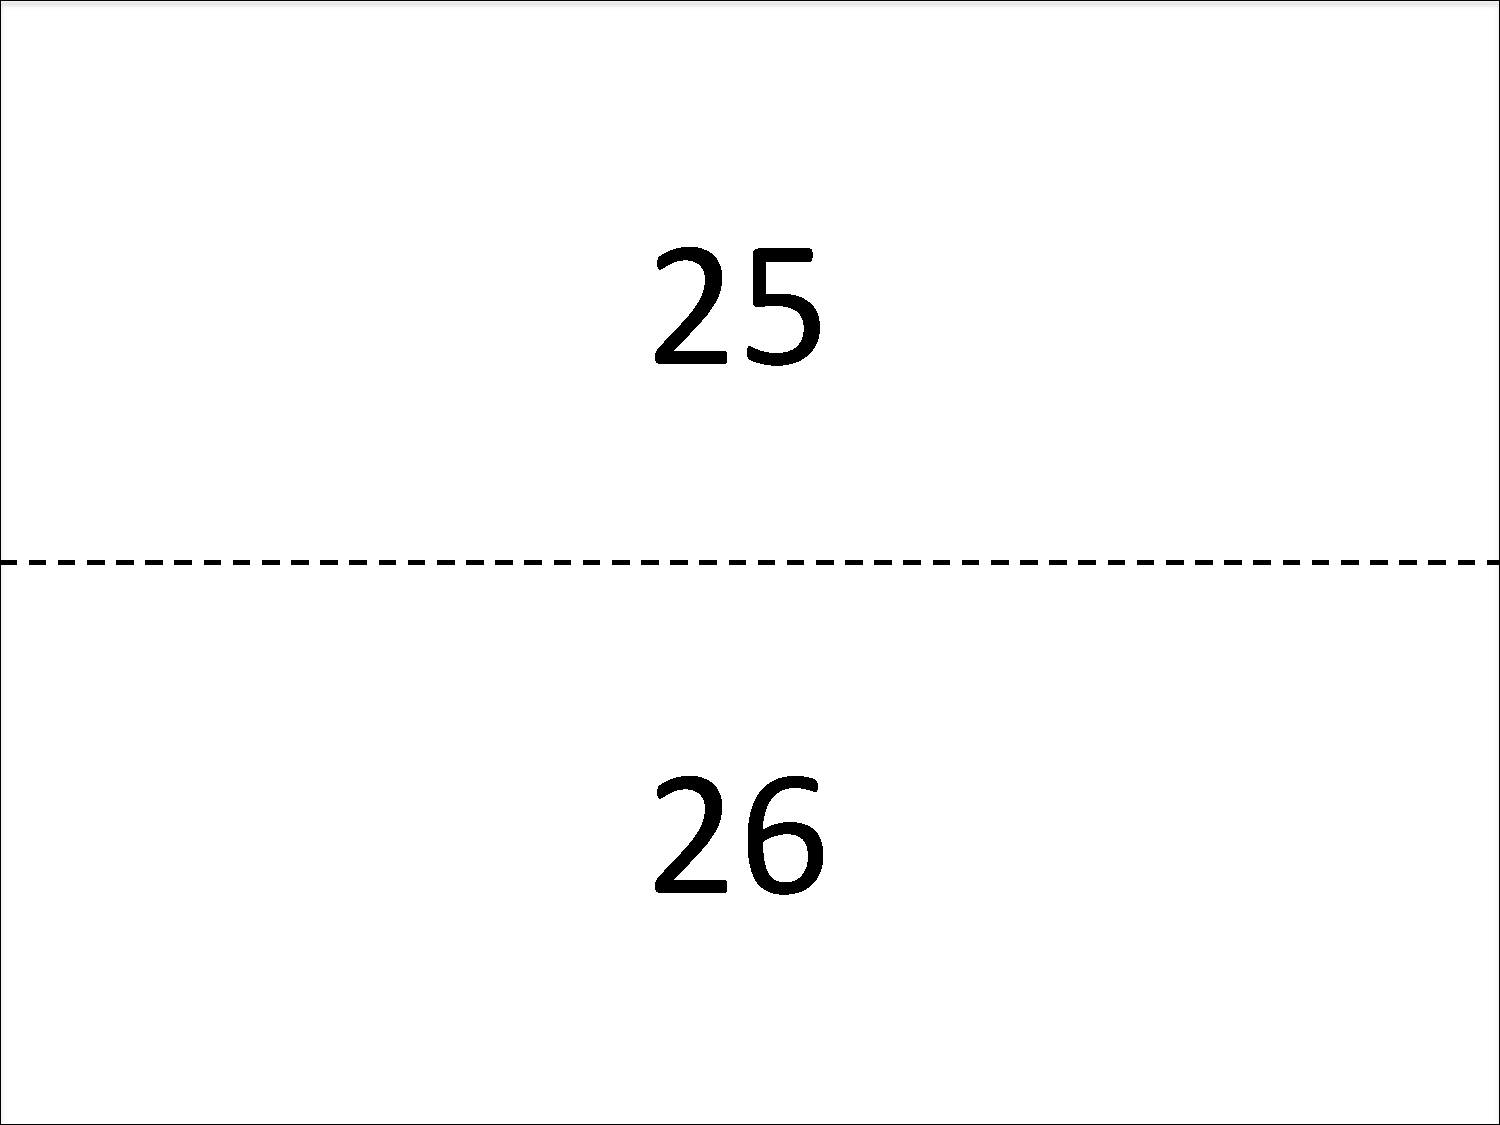
\includegraphics[width=0.19\textwidth]{images/partitioning2h.pdf}
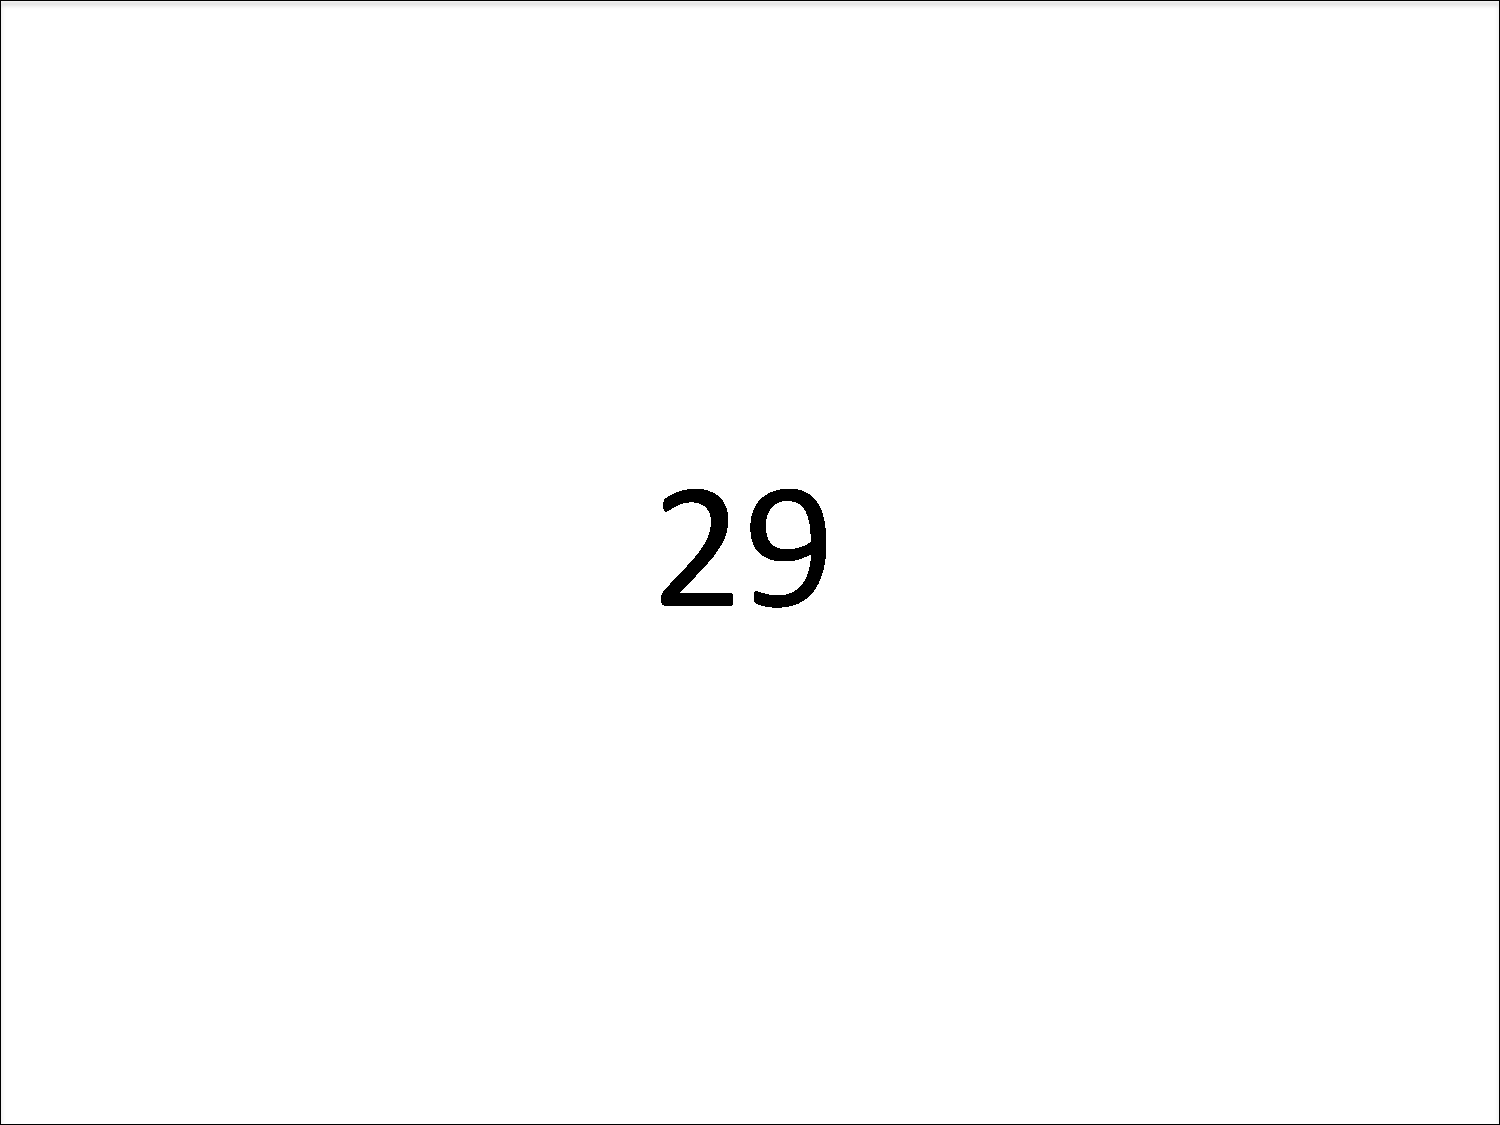
\includegraphics[width=0.19\textwidth]{images/partitioning1h.pdf}\vspace{1mm}
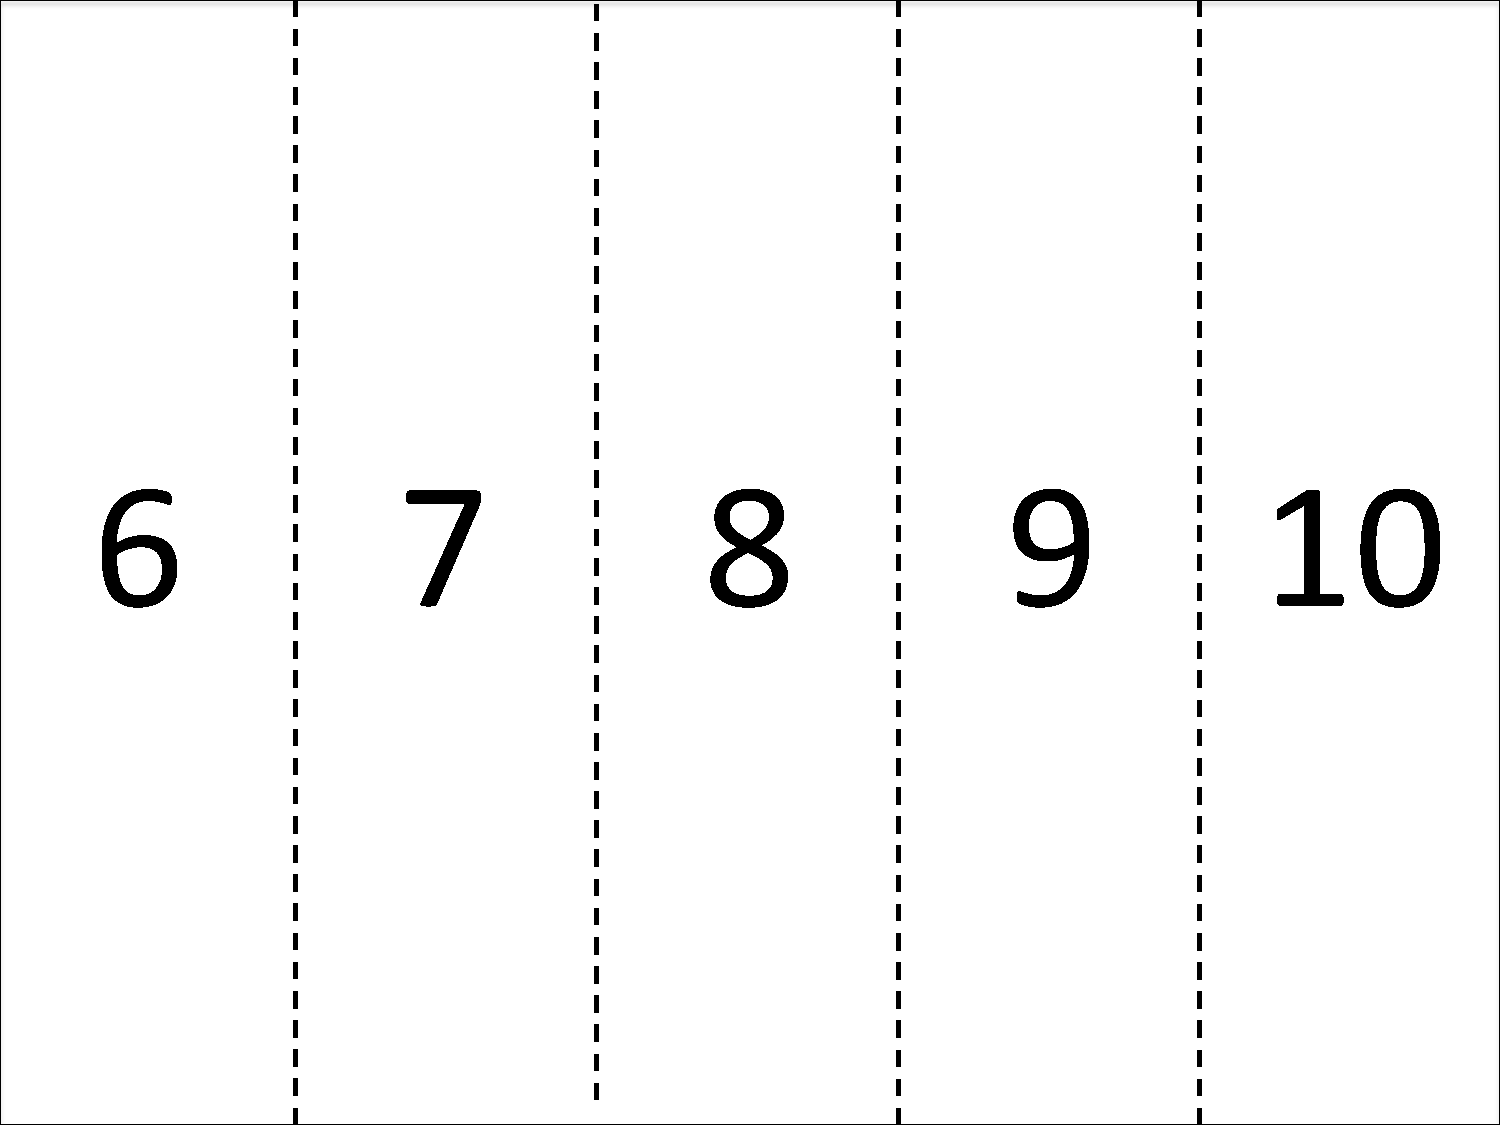
\includegraphics[width=0.19\textwidth]{images/partitioning5v.pdf}
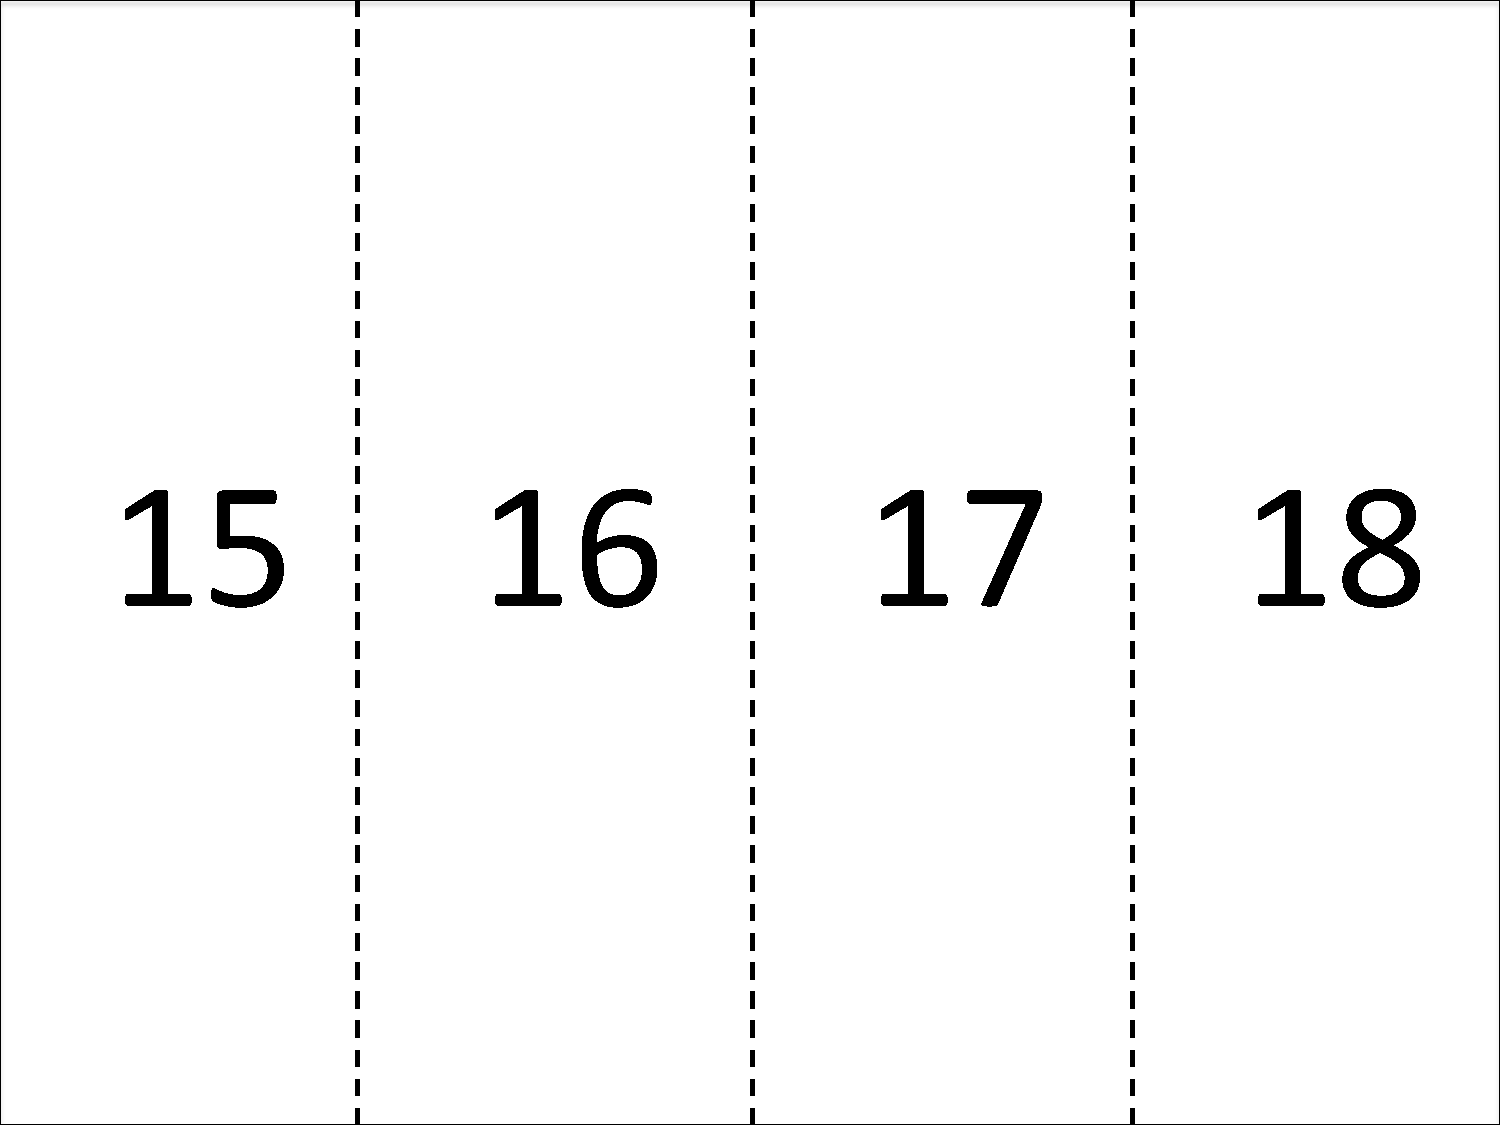
\includegraphics[width=0.19\textwidth]{images/partitioning4v.pdf}
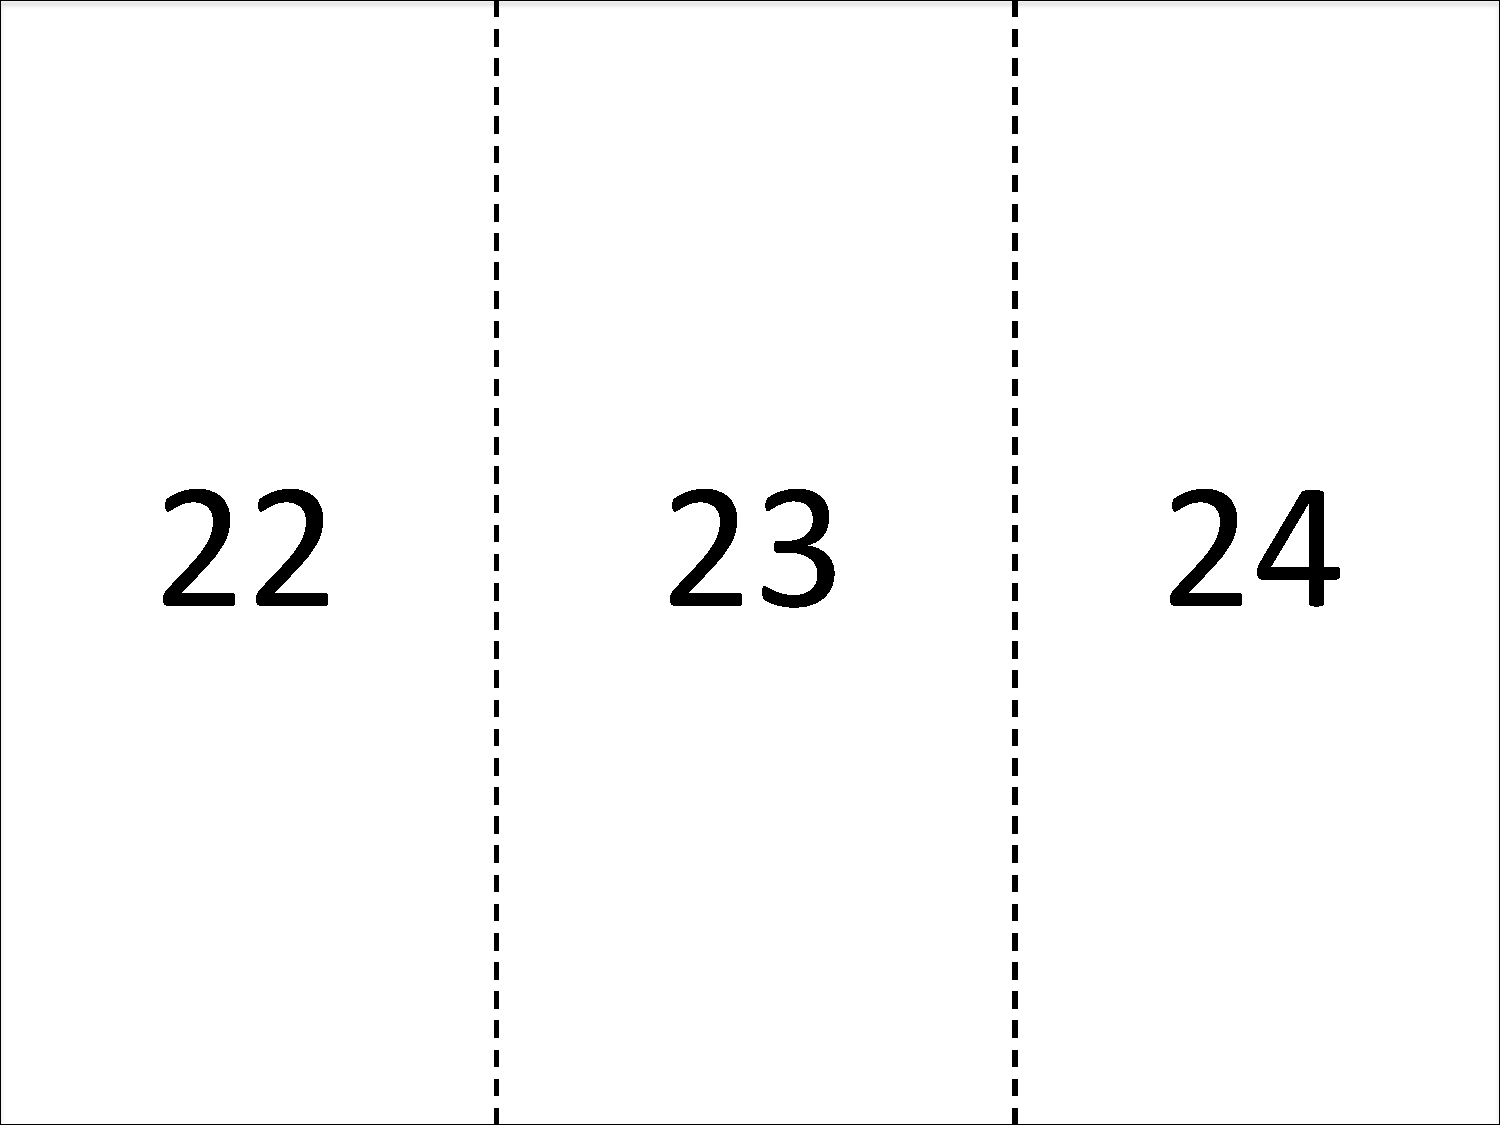
\includegraphics[width=0.19\textwidth]{images/partitioning3v.pdf}
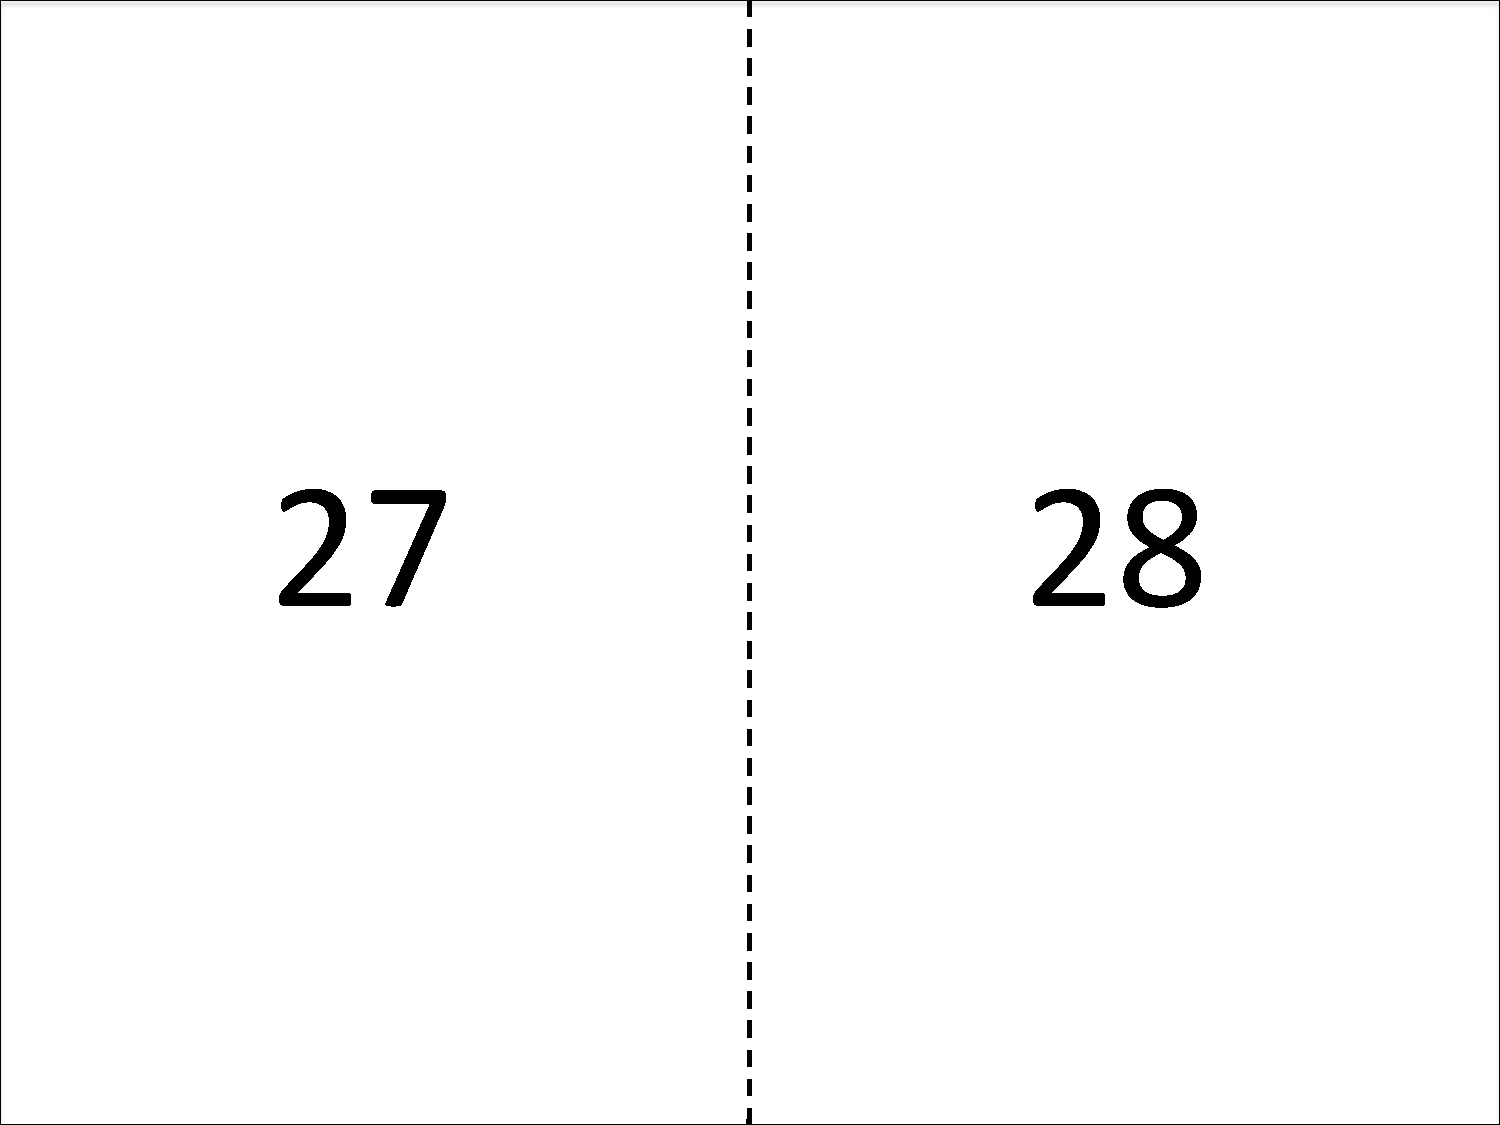
\includegraphics[width=0.19\textwidth]{images/partitioning2v.pdf}
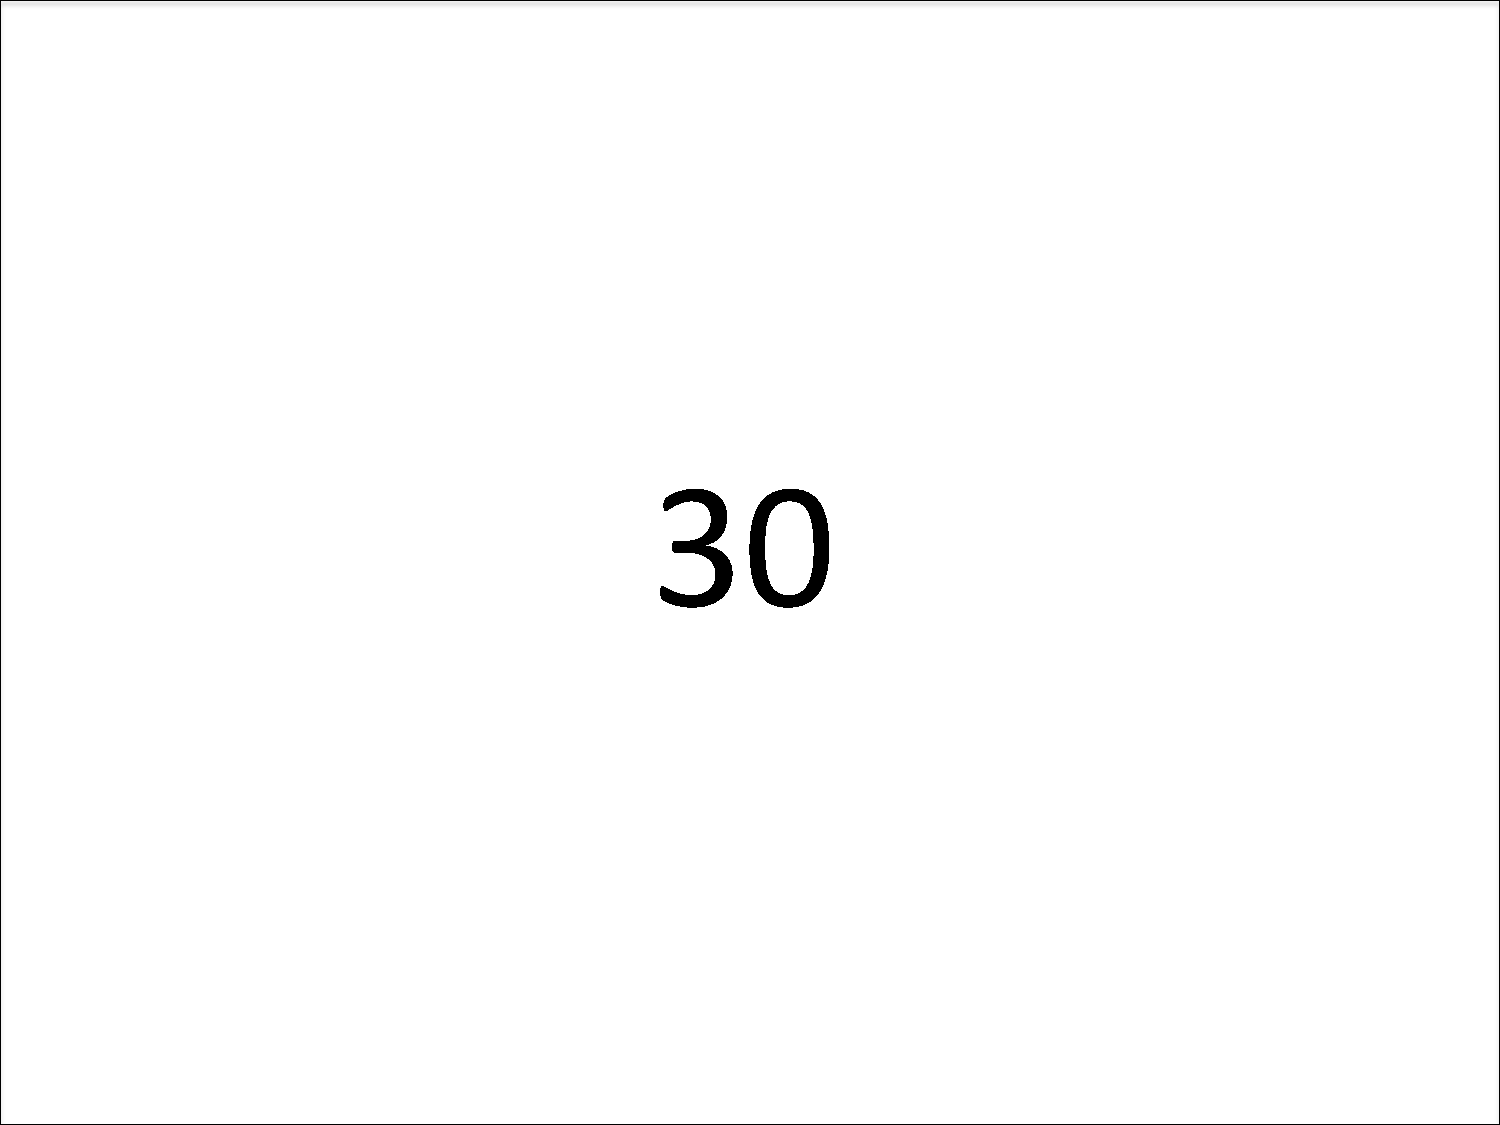
\includegraphics[width=0.19\textwidth]{images/partitioning1v.pdf}
\caption{Pyramidal image splitting for feature extraction}
\label{fig_blackwhite}
\end{figure}



\subsubsection{Clustering}
A first, rather naive approach to clustering the visual characteristics extracted would be to concatenate the feature vectors (histograms), and apply one of the established clustering algorithms like k-means. \index{K-Means} The fact that remains unseen in this approach is that, generally, the values of different features are usually measured on different scales and therefore vary in their orders of magnitude: In color histogram, each bin's value represents a number of pixels, whereas in edge histograms the number of edges is counted, which is significantly smaller. \\
This circumstances influences any algorithm based on the distance between two images. Since differences in the larger values will usually be larger in its absolute value, they will also be more influential to the overall distance than the dimensions with smaller values.

So, instead, we decided to apply k-means separately for colors and edges, and join the results later through \emph{late fusion}\index{Late Fusion}, as explained below. As no specific criteria exist for the number of clusters that should be achieved, k is chosen by the established rule of thumb: $ k = \sqrt{n/2} $ \cite[p.365]{mardia1979}, where n is the number of items to be clustered. K-means was chosen over hierarchical clustering, because it provided more well- and equally-sized clusters, the latter often just split off single images.\\
Initially, we planned to use an adaptive k, that is, start with a small k and increase it until the error (mean distance from centroids). Despite its higher computation complexity, it provides no better results than the rule of thumb. For example in color clustering, the adaptive approach will often just separate black and white images from colored ones.\\
We combine the single-feature clusters by intersecting them, which is a simple and performant late fusion method \index{Late Fusion}. It ensures that all images within a cluster are similar in color as well as edge structure and leads to less or equal to $ n/2 $ subclusters.
